\documentclass[letterpaper]{article} % DO NOT CHANGE THIS
\usepackage[submission]{aaai2027}  % DO NOT CHANGE THIS
\usepackage[hyphens]{url}  % DO NOT CHANGE THIS
\usepackage{graphicx} % DO NOT CHANGE THIS
\urlstyle{rm} % DO NOT CHANGE THIS
\def\UrlFont{\rm}  % DO NOT CHANGE THIS
\usepackage{natbib}  % DO NOT CHANGE THIS
\usepackage{caption} % DO NOT CHANGE THIS
\frenchspacing  % DO NOT CHANGE THIS
\usepackage{amsmath}
\usepackage{amssymb}
\usepackage{amsfonts}
\usepackage{bm}
\usepackage{booktabs}
\usepackage{multirow}

\pdfinfo{
/TemplateVersion (2027.1)
}

\setcounter{secnumdepth}{2}

\title{Response-Anchored Profile-to-PEFT: Turning a Handful of Answers into\\ Individual-Level Survey Personalization via Psychometric Graph Routing}

\author{
    Anonymous Submission
}
\affiliations{
    %
}

\begin{document}

\maketitle

\begin{abstract}
Large language models are increasingly used as synthetic survey respondents,
yet they are conditioned either on static demographic profiles or on nothing
at all, and reach only $30$--$40\%$ individual-level accuracy on large
sociological benchmarks. Demographic personas describe population-level
tendencies, not individuals: two respondents with identical age, education,
income, and country can hold opposite views, and a model conditioned only on
demographics cannot tell them apart. We ask whether a handful of a
respondent's real answers---as few as one to eight---can be turned into an
instant, parameter-level adaptation that a static demographic prior cannot
provide. We introduce \textbf{RAP2P} (Response-Anchored Profile-to-PEFT),
which routes a shared, rank-block-gated LoRA basis on a quantized $8$B
backbone using (i) a demographic prior conditioned on the target question and
(ii) a \emph{target-aware}, attention-weighted summary of the respondent's
known answers, biased by a leakage-safe item--item correlation graph estimated
from training respondents only. A prior-residual gate combines both signals
with an evidence weight that grows smoothly with the number of known answers,
producing a compact $64$-scalar per-(respondent, question) parameter state
without any per-respondent gradient step. On two SocioBench (ISSP) domains we
evaluate three generalization axes built from a single data partition---unseen
respondents, unseen demographic intersections, and unseen items---and
introduce \emph{Matched-Profile Heterogeneity}, a test of whether a model
distinguishes two demographically identical respondents whose true answers
diverge. Against demographic, classical-IRT, prompt-context, and
matched-capacity static-profile controls, RAP2P
\emph{[headline result: TBD once runs complete; see Table~\ref{tab:main}]}.
\end{abstract}

% \begin{links}
%     \link{Code}{https://github.com/Nicholas0027/RAP2P}
% \end{links}

\section{Introduction}

Survey research is expensive, slow, and increasingly plagued by declining
response rates, which has motivated a rapidly growing body of work that uses
large language models (LLMs) as synthetic respondents to anticipate or
supplement human answers \citep{bail2024generative,sarstedt2024using,heyde2024populi,suh2025language}.
The promise is attractive: if a model could reliably stand in for a
respondent, survey designers could pretest instruments, estimate subgroup
effects, and explore counterfactual populations at negligible cost. The
evidence, however, is sobering. When evaluated at the level of the individual
respondent rather than the aggregate marginal, current LLMs reach only
$30$--$40\%$ accuracy on large sociological benchmarks, and they exhibit
systematic distortions across demographic subgroups and sensitivity to
superficial prompt features such as option order
\citep{boelaert2025machine,williams2026beyond,bult2025llms}. A model that
matches a population's marginal distribution can still fail to reproduce its
joint structure, and a model that reproduces the joint structure can still
collapse every member of a demographic cell onto a single ``average'' opinion
\citep{williams2026beyond,wang2026parametric}.

The root difficulty is that a demographic persona describes a
\emph{population}, not a \emph{person}. Two respondents with identical age,
education, income, and country routinely hold opposing views, and a model
conditioned only on demographics has no signal that could separate them at
zero known answers. This suggests a different question from the one the
synthetic-respondent literature has largely asked. Rather than asking how
faithfully an LLM reproduces a demographic stereotype, we ask: given a
demographic prior \emph{and} a small number of a respondent's real answers,
can a lightweight, target-aware routing mechanism convert that sparse evidence
into an \emph{individual-level parameter adaptation} that neither a static
profile-to-parameter mapping nor an equivalent amount of in-context text can
achieve?

Two lines of work bracket this question. On one side, parameter-space
personalization maps a user descriptor directly to adapter weights: OPPU-style
per-user PEFT \citep{tan2024democratizing} and profile-to-parameter
hypernetworks \citep{mllereberstein2024hypernetworks,gupta2026amortizing}
generalize to unseen users without a per-user gradient step, but they encode a
\emph{static} profile that does not change with the question being asked. On
the other side, context-space personalization places the same information into
the prompt as text, inheriting the token cost and option-order fragility that
plague survey LLMs \citep{boelaert2025machine}. Neither line exploits a
structural fact specific to surveys: items are correlated, so the relevance of
a known answer to a target question is not uniform---knowing a respondent's
view on carbon taxation is highly informative for a related environmental item
and nearly irrelevant for a national-pride item. RAP2P is built around exactly
this inductive bias.

We introduce \textbf{Response-Anchored Profile-to-PEFT (RAP2P)}. On the last
$L$ decoder layers of a quantized $8$B backbone, RAP2P maintains one
population-shared LoRA basis of rank $R=B\times r$, decomposed into $B$
rank-$r$ blocks and mixed per (respondent, question) by a softmax gate. The
gate is driven by a \emph{prior-residual} combination of a
question-conditioned demographic prior and a \emph{target-aware}
attention summary of the respondent's $K$ known answers, in which the
attention score is biased by a leakage-safe item--item correlation graph
estimated only on training respondents. An evidence weight
$\rho_K = K/(K+\tau)$ damps the response-anchoring branch to zero when no
answers are available and lets it grow smoothly as answers accumulate. The
personalized state per (respondent, question) is only $L\times M\times B$
scalars---$64$ values in our configuration---and requires no per-respondent
optimization at inference time.

We make three contributions.
\begin{itemize}
\item \textbf{RAP2P}, a shared rank-block-gated LoRA basis routed by a
prior-residual gate that fuses a question-conditioned demographic prior with a
target-aware, psychometric-graph-biased summary of a respondent's few known
answers (Section~\ref{sec:method}).
\item \textbf{A controlled experimental design from a single data partition}
that isolates three generalization axes (unseen respondent, unseen demographic
intersection, unseen item) and a capacity-matched static-profile control,
pinning down precisely what target-aware routing adds over a static
profile-to-parameter mapping and over the same information delivered as prompt
tokens (Section~\ref{sec:setup}).
\item \textbf{Matched-Profile Heterogeneity}, an evaluation that directly
tests whether a model differentiates demographically identical respondents
whose true answers diverge---a sharp test of ``not a stereotype machine''
(Section~\ref{sec:hetero}).
\end{itemize}

We deliberately scope the study to two SocioBench domains and state the axes we
drop (cross-country generalization, an exhaustive per-loss-term ablation)
explicitly rather than silently (Section~\ref{sec:limitations}).

\section{Related Work}
\label{sec:related}

\paragraph{LLMs as synthetic survey respondents.}
The idea of substituting LLM outputs for human survey responses has moved
quickly from proof-of-concept to critical scrutiny. Recent work builds
individual-grounded agents from self-reports \citep{park2024agents},
fine-tunes on large-scale survey corpora to predict opinion distributions
\citep{suh2025language}, and evaluates cross-cultural transfer of opinion
simulation across Chinese and U.S. models \citep{qi2025crosscultural}. At the
same time, methodological audits report that generative models answer opinion
polls with pronounced machine biases \citep{boelaert2025machine}, that
distributional and individual-level accuracy diverge sharply
\citep{miranda2025simulating}, and that estimates of national public opinion
are sensitive to prompt language and framing
\citep{heyde2024populi,bult2025llms}. Our work departs from the dominant
persona-prompting paradigm along the individual-level axis: rather than
steering a frozen model with a demographic description, we route
parameter-space adaptation from a small number of the respondent's own
answers.

\paragraph{Representativeness beyond marginals.}
A recurring finding is that matching a population's single-item marginal
distribution does not imply matching its joint (item--item) correlation
structure, and that demographic conditioning can produce ``flattened''
subpopulations that erase within-group heterogeneity
\citep{williams2026beyond,wang2026parametric}. This motivates two of our
evaluation axes: an expected-score item--item correlation-fidelity test
(Table~\ref{tab:structure}) and Matched-Profile Heterogeneity
(Table~\ref{tab:hetero}), which asks whether the model keeps two
demographically identical but behaviorally divergent respondents apart. We
measure structural fidelity rather than optimizing for it, so that any observed
fidelity is emergent rather than trained in.

\paragraph{Personalized parameter-efficient fine-tuning.}
Personalizing LLMs through PEFT has been approached either by learning a
separate adapter per user---OPPU-style personalized PEFT
\citep{tan2024democratizing}---or by amortizing adaptation through a
hypernetwork that maps a user descriptor directly to adapter weights
\citep{mllereberstein2024hypernetworks,gupta2026amortizing,otsuka2024userspecific}.
Amortized approaches avoid a per-user gradient step and generalize to unseen
users, which is the property we require, but they encode a \emph{static}
descriptor: the mapping from profile to parameters does not change with the
question being asked. RAP2P keeps the ``no per-user gradient step'' property
while making the routing \emph{target-aware}, recomputing the
response-anchoring summary for every target item. Our capacity-matched
static-profile control (Section~\ref{sec:baselines}) isolates precisely this
difference.

\paragraph{Mixtures of LoRA experts and routed adapters.}
Architecturally, our rank-block gating is a mixture of low-rank experts: a
shared basis is partitioned into rank blocks combined by a per-example gate,
as in X-LoRA \citep{buehler2024xlora}, block-wise and rank-wise LoRA mixtures
\citep{li2024blockwise,zou2025flylora}, asymmetric shared-basis designs
\citep{tian2024hydralora}, and recent routed-adapter methods with learned or
attention-based routing \citep{li2025loramixer,zhuang2025ldmole,ban2026rethinking}.
The generic PEFT and LoRA-mixture literature is surveyed in
\citet{han2024parameterefficient} and refined by decomposition- and
learning-rate-aware variants \citep{liu2024dora,lee2026learning}. Our
contribution is not the mixing mechanism but \emph{what drives the gate}: a
demographic prior and a target-aware, psychometrically biased summary of a
respondent's own answers, rather than a task embedding or a data-driven cluster
assignment. To our knowledge, no prior LoRA-mixture method conditions the gate
on an item--item correlation graph estimated from the response matrix itself.

\section{Method}
\label{sec:method}

\begin{figure*}[t]
\centering
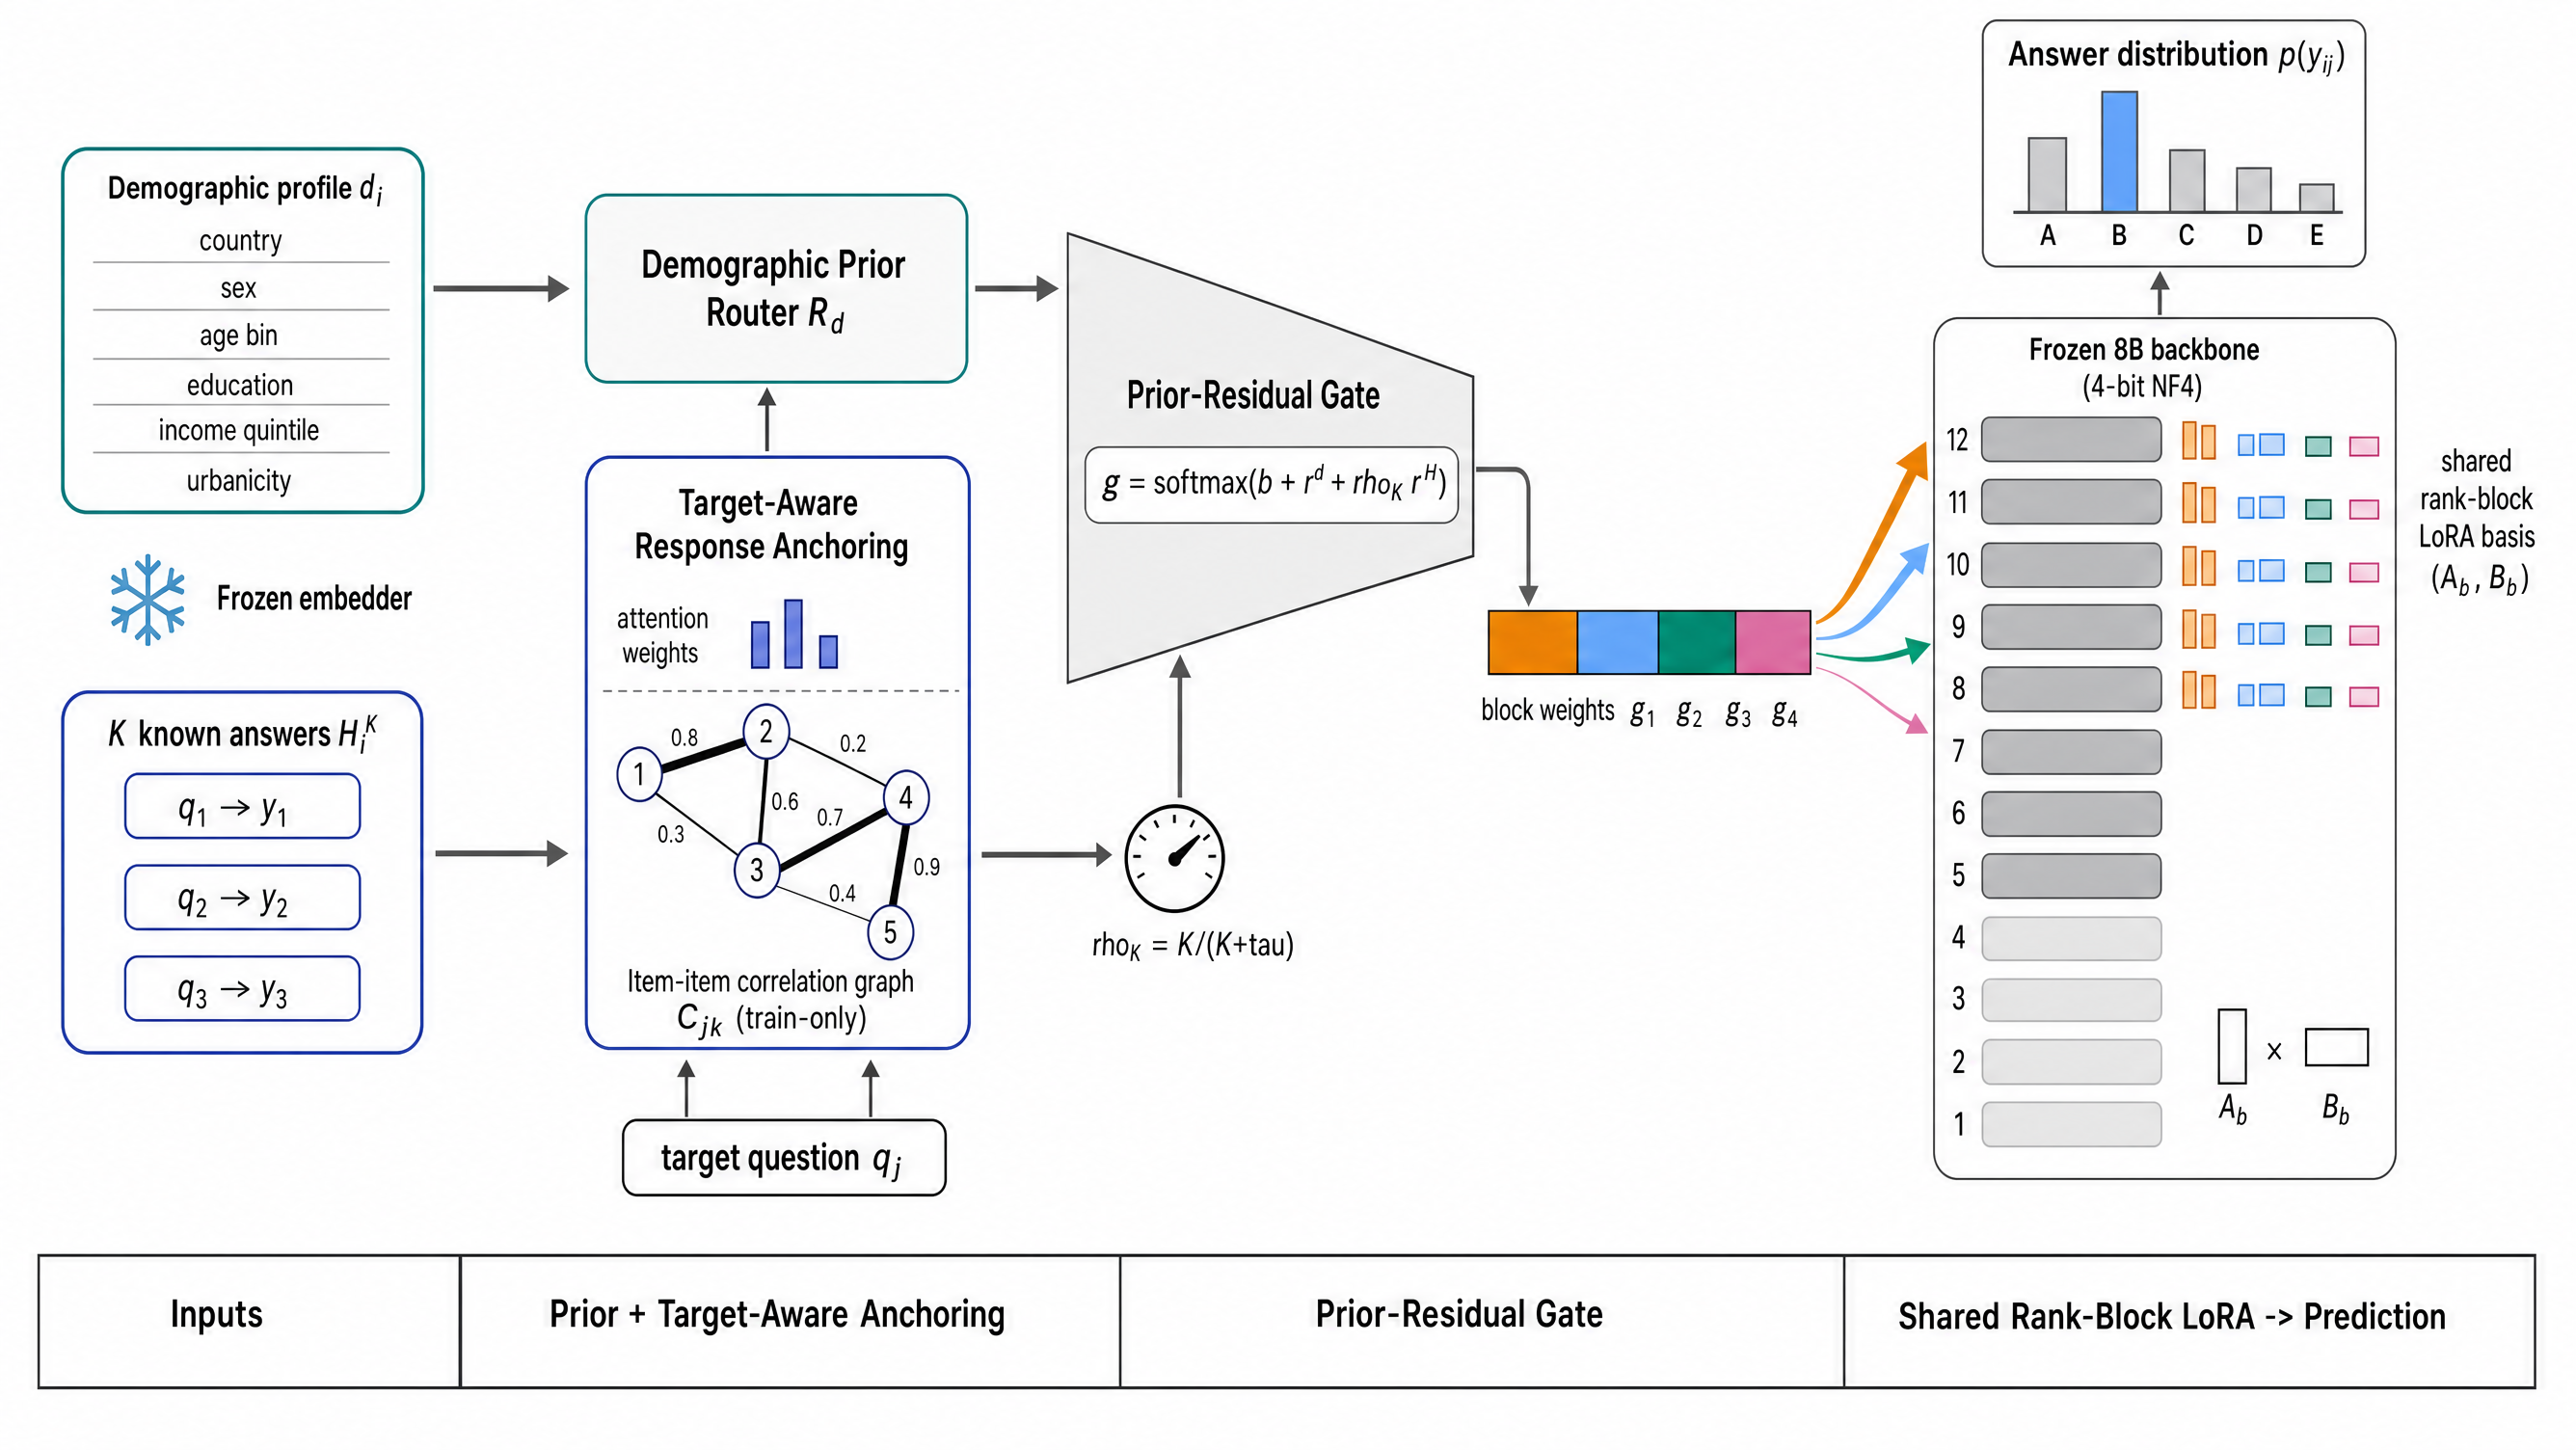
\includegraphics[width=0.94\textwidth]{figures/fig1_architecture.png}
\caption{The RAP2P architecture. A demographic prior router and a
target-aware response-anchoring branch---the latter biased by a leakage-safe
item--item correlation graph $C_{jk}$ estimated on training respondents
only---are both conditioned on the target question $q_j$ and combined by a
prior-residual gate. An evidence weight $\rho_K = K/(K+\tau)$ damps the
response-anchoring contribution toward zero when few answers are known. The
gate produces a $B$-way mixture over a shared rank-block LoRA basis
$\{(\bm{A}_b,\bm{B}_b)\}$ applied to the last eight layers of a frozen $4$-bit
$8$B backbone, yielding a per-(respondent, question) prediction with only
$L\times M\times B = 64$ personalized scalars and no per-respondent gradient
step.}
\label{fig:arch}
\end{figure*}

\subsection{Problem statement}
For an unseen respondent $i$ with demographics $d_i$, a set of $K$ known
question--answer pairs $H_i^K = \{(q_k, y_{ik})\}_{k=1}^{K}$, and a target
question $q_j$, we predict the answer distribution
\begin{equation}
p\big(y_{ij} \mid d_i, H_i^K, q_j\big)
\label{eq:problem}
\end{equation}
without any per-respondent gradient update. The number of known answers
$K\in\{0,1,3,5,8\}$ is sampled per training batch (variable-$K$ training, so a
single checkpoint covers every $K$) and held fixed within an evaluation pass.
At $K=0$ the task reduces to demographic-only prediction; as $K$ grows the
model should behave more like the specific individual and less like the
demographic average.

\subsection{Shared rank-block-gated LoRA basis}
On the backbone's last $L$ decoder layers, for each of $M$ target modules
(\texttt{q\_proj}, \texttt{v\_proj}), we maintain one population-shared LoRA of
rank $R=B\times r$, split along the rank dimension into $B$ blocks
$\{(\bm{A}_b, \bm{B}_b)\}_{b=1}^{B}$. The per-example weight update is a
gated sum of the block contributions,
\begin{equation}
\Delta \bm{W}^{(l,m)} = \sum_{b=1}^{B} g_b^{(l,m)}\, \bm{B}_b^{(l,m)} \bm{A}_b^{(l,m)},
\qquad \bm{g}^{(l,m)} = \mathrm{softmax}(\cdot)\in\Delta^{B-1},
\label{eq:gatedlora}
\end{equation}
computed without materializing a per-example full-rank matrix: $\bm{A}$ is
applied once across concatenated blocks, the gate scales the low-rank
intermediate per block, and $\bm{B}$ is applied once. Every respondent shares
the \emph{same} basis atoms $(\bm{A}_b, \bm{B}_b)$; only the $B$-dimensional
mixture weight is personalized. The per-(respondent, question) parameter state
is therefore just $L\times M\times B$ scalars---with $L{=}8$, $M{=}2$, $B{=}4$,
exactly $\mathbf{64}$ values, versus the tens of millions of parameters a
per-user adapter would carry.

\subsection{Prior-residual gate}
The gate logits for layer $l$, module $m$, respondent $i$, target $j$ combine
a population default, a demographic prior, and a response-anchoring residual:
\begin{equation}
\bm{g}_{ij}^{(l,m)} = \mathrm{softmax}\!\Big[\, \bm{b}^{(l,m)}
   + \bm{r}_{ij}^{d,(l,m)}
   + \rho_{K_i}\, \bm{r}_{ij}^{H,(l,m)} \,\Big],
\qquad
\rho_{K_i} = \frac{K_i}{K_i + \tau},
\label{eq:gate}
\end{equation}
with $\tau{=}2$. Here $\bm{b}^{(l,m)}$ is a learned, respondent-independent
bias---the population default that dominates at $K{=}0$ with uninformative
demographics; $\bm{r}_{ij}^{d}$ is the demographic prior router
(Section~\ref{sec:demoprior}); and $\bm{r}_{ij}^{H}$ is the target-aware
response-anchoring summary (Section~\ref{sec:anchoring}), damped by
$\rho_{K_i}$ so it contributes nothing when no answers are available and grows
smoothly as answers accumulate. Crucially, $K_i$ is each respondent's
\emph{actual} number of known answers in the batch (read from the history
mask, not the batch's nominal $K$): a respondent with fewer answered items than
the sampled $K$ receives a correspondingly smaller evidence weight.

\subsection{Demographic prior router}
\label{sec:demoprior}
The demographic contribution conditions on both the respondent and the target
question,
\begin{equation}
\bm{r}_{ij}^{d} = R_d\big(\big[\,\bm{h}_i^d \,;\, \pi(\bm{e}_j)\,\big]\big),
\qquad
\bm{h}_i^d = \mathrm{MLP}\big(\mathrm{Embed}_{\mathrm{frozen}}(\text{demographic text}_i)\big),
\label{eq:demo}
\end{equation}
where $\bm{h}_i^d$ is a small trainable MLP over a \emph{frozen} sentence
embedding of the respondent's formatted demographic string (country, sex, age
bin, education, income quintile, employment, marital status, urbanicity), and
$\bm{e}_j$ is the frozen embedding of the target question passed through a
learned projection $\pi$ before concatenation. Conditioning on the target item
lets the same demographic profile push the gate differently depending on the
question: income should matter more for a taxation item than for a
national-pride item.

\subsection{Target-aware response anchoring}
\label{sec:anchoring}
This is the central mechanism. Each known answer is encoded as
\begin{equation}
\bm{r}_{ik} = \mathrm{MLP}\big(\big[\,\bm{e}_k \,;\, E_y(y_{ik})\,\big]\big),
\label{eq:answerenc}
\end{equation}
where $\bm{e}_k$ is the frozen embedding of known question $k$ and $E_y$ is a
small \emph{trainable} answer-position embedding---the model learns how much an
answer's ordinal position should shift the representation, rather than baking
it into a frozen text encoder. The $K$ known answers are aggregated by an
attention score that mixes learned semantic similarity with a precomputed,
leakage-safe item--item correlation prior $C_{jk}$:
\begin{align}
\alpha_{ijk} &= \mathrm{softmax}_k\!\left[\,
   \frac{(\bm{W}_q \bm{e}_j)^{\!\top} (\bm{W}_k \bm{e}_k)}{\sqrt{d}}
   + \gamma\, C_{jk} \,\right],
\label{eq:attn}\\
\bm{h}_{i\to j}^{H} &= \sum_{k=1}^{K}\alpha_{ijk}\, \bm{r}_{ik},
\qquad
\bm{r}_{ij}^{H} = R_h\big(\bm{h}_{i\to j}^{H}\big).
\label{eq:anchor}
\end{align}
The correlation prior $C_{jk}$ is a shrinkage-corrected Spearman correlation
between items $j$ and $k$, estimated \emph{only} on training-split respondents,
\begin{equation}
C_{jk} = \frac{n_{jk}}{n_{jk}+\lambda}\;\rho_{\mathrm{Spearman}}(q_j, q_k),
\qquad \lambda{=}50,
\label{eq:corr}
\end{equation}
with $C_{jk}$ set to zero whenever the co-answering count $n_{jk}$ falls below a
minimum threshold. Equation~\eqref{eq:attn} is the paper's central inductive
bias: the \emph{same} $K$ known answers are weighted differently depending on
what is being predicted, using the survey's own item structure as a prior on
relevance. This is exactly the signal a static profile encoder discards, since
it summarizes the $K$ answers once, identically, regardless of the target
question---the behavior of our P2P-Static control (Section~\ref{sec:baselines}).

\subsection{Training objective}
We train with two loss terms only, reading solely the option-label token
logits (\texttt{A}\dots\texttt{J}):
\begin{equation}
\mathcal{L} = \mathcal{L}_{\mathrm{CE}} + \lambda_{\mathrm{ord}}\,\mathcal{L}_{\mathrm{ord}},
\qquad
\mathcal{L}_{\mathrm{ord}} = \frac{1}{n_{\mathrm{opt}}-1}\sum_{c} p(c)\,\lvert c - y_{ij}\rvert,
\label{eq:loss}
\end{equation}
with $\lambda_{\mathrm{ord}}{=}0.1$. The ordinal term penalizes predictions
that are far from the true option on the Likert scale, not merely wrong. The
label-to-option mapping is re-randomized every epoch during training and
averaged over fixed permutations at test time (Section~\ref{sec:robustness}).
A router-collapse guard adds $\lambda_{\mathrm{bal}}\sum_b(\bar g_b - 1/B)^2$
\emph{only if} triggered (any block's mean gate share exceeds a threshold), so
it does not appear in the loss of a healthy run. We deliberately add \emph{no}
KL, marginal-distribution, or structural-correlation loss term: the structural
fidelity reported in Table~\ref{tab:structure} is therefore an emergent
property of accurate individual-level modeling, not a directly optimized
target---a stronger and more falsifiable claim than training the correlation
structure in and reading it back out.

\subsection{Modality dropout and training-time ``free'' ablations}
During RAP2P's main training run, the demographics, history, and correlation
signals are independently dropped per example with probabilities
$0.20$, $0.20$, $0.15$. Because the model learns to function with any subset of
these signals missing, most ablation rows (no-demographics, no-history,
no-correlation-graph, uniform-gate) can be produced at \emph{inference} time on
the single trained checkpoint by hard-zeroing the corresponding keep-mask,
rather than retraining a separate model for each. This is a compute-saving
methodological choice, not a free lunch: we retrain one ablation from scratch
(RAP2P-noGraph, with $\gamma$ fixed to zero at construction) and a cross-check
(RAP2P-noHistory-retrained) to confirm the inference-time ablations track what
a true retrain would show (Section~\ref{sec:ablations}).

\section{Experimental Setup}
\label{sec:setup}

\subsection{Data}
We use two SocioBench (ISSP) domains: \emph{Environment} and \emph{Role of
Government}. Per domain we retain the $20$ highest-coverage ordinal items and
keep respondents from every sampled country, capping at $3{,}000$ respondents
per country and dropping respondents with fewer than $12$ answered (kept)
items. The curation rule is frozen before any modeling and does not depend on
any model's predictions. Table~\ref{tab:data} summarizes the resulting corpus;
\emph{[NOTE: fill counts from} \texttt{artifacts/processed/audit.json}
\emph{---the} \texttt{curation} \emph{and} \texttt{leakage} \emph{blocks give
kept items/countries, per-split panel counts, and total rows.]}

\begin{table}[t]
\centering
\caption{Corpus after curation and leakage-safe splitting. Counts are filled
from \texttt{artifacts/processed/audit.json}. ID = unseen-respondent test;
OOD-Int = unseen demographic-intersection holdout; unseen items are excluded
from all calibration histories and training targets.}
\label{tab:data}
\begin{tabular}{lcc}
\toprule
 & Environment & Role of Gov. \\
\midrule
Countries kept              & [--] & [--] \\
Items kept (unseen: 15\%)   & [--] & [--] \\
Train respondents           & [--] & [--] \\
Validation respondents      & [--] & [--] \\
ID test respondents         & [--] & [--] \\
OOD-Int respondents         & [--] & [--] \\
Total (resp.\,$\times$\,item) rows & [--] & [--] \\
\bottomrule
\end{tabular}
\end{table}

\subsection{Three generalization axes from one partition}
All three axes derive from a single split assignment, not three separate
re-splits, so differences across axes are not confounded by different training
data.
\begin{itemize}
\item \textbf{ID --- Unseen Respondent}: a standard $70/10/20$ respondent-level
split, stratified by domain, country, sex, and age bin.
\item \textbf{OOD --- Unseen Intersection}: demographic cells (age-bin
$\times$ education $\times$ income-quintile $\times$ urbanicity) with enough
respondents are held out \emph{entirely}, so every respondent in a held-out
cell is removed from train/validation/test. Training still observes every
individual attribute value, just never that exact combination.
\item \textbf{OOD --- Unseen Item}: $15\%$ of kept items per domain are
excluded from every respondent's calibration history and from all training
targets; they appear only as test-time targets. A leakage guard asserts this
holds before any GPU time is spent.
\end{itemize}

\subsection{Baselines}
\label{sec:baselines}
Table~\ref{tab:baselines} lists the comparison methods, chosen to isolate the
contribution of target-aware routing from cheaper explanations.

\begin{table}[t]
\centering
\caption{Baselines and their inputs. $d$ = demographics, $q$ = target
question, $H_i^K$ = $K$ known answers. Trained methods share the same backbone,
target modules, and total rank as RAP2P.}
\label{tab:baselines}
\setlength{\tabcolsep}{4pt}
\begin{tabular}{llc}
\toprule
ID & Method & Input \\
\midrule
B0 & Majority                       & $q$ \\
B1 & Demographic Frequency          & $d,q$ \\
B2 & Question Frequency             & $q$ \\
B3 & Demographic MIRT               & $d,H_i^K,q$ \\
B4 & Local-8B Persona               & $d,q$ \\
B5 & Local-8B Sparse-ICL            & $d,H_i^K,q$ \\
B6 & Strong-API Sparse-ICL          & $d,H_i^K,q$ \\
B7 & Global QLoRA                   & $d,q$ \\
B8 & Context QLoRA                  & $d,H_i^K,q$ (prompt) \\
B9 & P2P-Static                     & $d,H_i^K$ (static route) \\
\textbf{Ours} & \textbf{RAP2P}      & $d,H_i^K,q$ (target route) \\
\bottomrule
\end{tabular}
\end{table}

B3 (Demographic MIRT) is the classical latent-trait comparison point: if it
matches RAP2P, the gain comes from a classical prior--posterior update, not
from LLM item semantics or target-aware routing. B7/B8 use a standard
contiguous LoRA of the same total rank, alpha, and target modules as RAP2P's
basis (matched capacity, not block-gated). B9 (P2P-Static) shares RAP2P's exact
rank-block architecture, router hidden size, and warm-started basis, isolating
precisely the target-conditioned-routing difference; it is a
\emph{P2P-style static-profile control}, not a reproduction of any published
hypernetwork stack. B6 uses a strong hosted chat model on a fixed
$500$-respondent stratified subsample; its probabilities are a hard-label
approximation (no logprob access), so we report accuracy and ordinal MAE as
primary and flag NLL/Brier as approximate. Global/Context QLoRA and all
rank-block methods receive the \emph{same} text prompt (demographics plus
target question, no history text) except Context QLoRA, whose purpose is to
test in-context personalization---this equalizes the text channel across every
method except the one built to probe it.

\subsection{Training matrix and seeds}
Global QLoRA and Context QLoRA are trained with seeds $\{1701, 7\}$; RAP2P with
$\{1701, 7, 42\}$; P2P-Static with $\{1701, 7\}$; and the two retrained
ablations (RAP2P-noGraph, RAP2P-noHistory-retrained) with seed $1701$. The
Global QLoRA checkpoint \emph{warm-starts} every rank-block basis run: the
contiguous rank-$16$ adapter is split into $4$ blocks with $\bm{B}$ scaled by
$B$, so the initial $\Delta\bm{W}$ under a uniform gate reproduces the Stage-1
adapter exactly. All rank-block runs share the same two-tier learning rate
(router $5\!\times\!10^{-4}$, basis $2\!\times\!10^{-5}$) and the same warm
start, so no ablation gap can be attributed to a learning-rate or
initialization mismatch. The backbone is Llama-3.1-8B-Instruct under $4$-bit
NF4 quantization with adapters on the last $8$ layers' \texttt{q\_proj} and
\texttt{v\_proj}; the full training matrix fits in roughly $75$--$110$
GPU-hours on a single $24$\,GB GPU. \emph{[NOTE: report realized GPU-hours and
per-run steps-to-convergence from} \texttt{artifacts/checkpoints/*/history.json}
\emph{in the camera-ready.]}

\subsection{Robustness and statistics}
\label{sec:robustness}
We report three robustness/statistical protocols. \textbf{Option-order
robustness}: five option-permutation seeds re-run over a fixed
$500$-respondent subsample of the ID test split; we report semantic-answer
permutation consistency, the fraction of (respondent, item) pairs whose
predicted answer is stable across all five permutations
(Table~\ref{tab:permutation}). \textbf{Respondent-level paired bootstrap}:
$2{,}000$ resamples, grouped by domain and panel, giving $95\%$ confidence
intervals on accuracy differences (Table~\ref{tab:bootstrap}). \textbf{Holm
correction} at $\alpha{=}0.05$ across the family of
method-vs-Context-QLoRA, method-vs-P2P-Static, and method-vs-MIRT comparisons
at every $K$.

\section{Results}
\label{sec:results}

All numeric cells below are placeholders (\texttt{[--]}) until the training and
evaluation runs complete; each table caption states the exact source file and
column so that filling the draft is a copy operation, not a rewrite. Unless
noted, results are macro-averaged over the two domains and averaged over seeds,
with the ID test split and \texttt{item\_pool=seen}.

\subsection{Few-response personalization (Table~\ref{tab:main})}
Table~\ref{tab:main} is the headline result: individual-level accuracy as a
function of the number of known answers $K$. AUAC is the unweighted mean
accuracy over the (unevenly spaced) grid $K\in\{0,1,3,5,8\}$, and $\Delta_5$ is
accuracy$(5)-$accuracy$(0)$, the personalization lift from five answers.

\begin{table*}[t]
\centering
\caption{Few-response personalization on the ID test split (macro domain,
seen items). Accuracy at each $K$; AUAC = mean accuracy over the $K$ grid;
MAE and NLL at $K{=}5$. \emph{Source:}
\texttt{artifacts/metrics/table1\_main.csv} (columns \texttt{acc\_k0..acc\_k8},
\texttt{auac}, \texttt{mae\_k5}, \texttt{nll\_k5}); rows are one per method
after seed aggregation. Report mean$\pm$std over seeds using
\texttt{respondent\_macro\_seed\_mean.csv} (\texttt{accuracy\_std}). Bold the
best in each column. B6 (Strong-API) is on a 500-respondent subsample; report
its parse-failure rate in a footnote.}
\label{tab:main}
\setlength{\tabcolsep}{5pt}
\begin{tabular}{lccccccccc}
\toprule
Method & $K{=}0$ & $K{=}1$ & $K{=}3$ & $K{=}5$ & $K{=}8$ & AUAC\,$\uparrow$ & $\Delta_5\,\uparrow$ & MAE$_5\,\downarrow$ & NLL$_5\,\downarrow$ \\
\midrule
Majority                    & [--] & [--] & [--] & [--] & [--] & [--] & [--] & [--] & [--] \\
Demographic Frequency       & [--] & [--] & [--] & [--] & [--] & [--] & [--] & [--] & [--] \\
Question Frequency          & [--] & [--] & [--] & [--] & [--] & [--] & [--] & [--] & [--] \\
Demographic MIRT            & [--] & [--] & [--] & [--] & [--] & [--] & [--] & [--] & [--] \\
Local-8B Persona            & [--] & [--] & [--] & [--] & [--] & [--] & [--] & [--] & [--] \\
Local-8B Sparse-ICL         & [--] & [--] & [--] & [--] & [--] & [--] & [--] & [--] & [--] \\
Strong-API Sparse-ICL$^{\dagger}$ & [--] & [--] & [--] & [--] & [--] & [--] & [--] & [--] & [--] \\
Global QLoRA                & [--] & [--] & [--] & [--] & [--] & [--] & [--] & [--] & [--] \\
Context QLoRA               & [--] & [--] & [--] & [--] & [--] & [--] & [--] & [--] & [--] \\
P2P-Static                  & [--] & [--] & [--] & [--] & [--] & [--] & [--] & [--] & [--] \\
\textbf{RAP2P}              & [--] & [--] & [--] & [--] & [--] & [--] & [--] & [--] & [--] \\
\bottomrule
\end{tabular}
\end{table*}

The adaptation curves are visualized in Figure~\ref{fig:curve}: RAP2P should
start near the demographic baselines at $K{=}0$ and separate from Context
QLoRA and P2P-Static as $K$ grows, if target-aware routing converts sparse
evidence into individual-level lift. \emph{[NOTE: go/no-go reading---if RAP2P
does not clear Context QLoRA at $K\in\{3,5\}$ by a bootstrap-significant margin
(Table~\ref{tab:bootstrap}), report the graceful-degradation framing in
Section~\ref{sec:discussion} rather than overclaiming.]}

\begin{figure}[t]
\centering
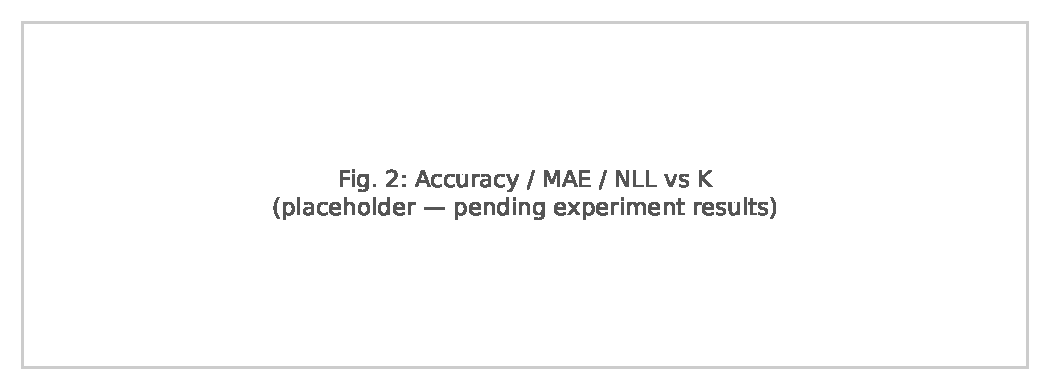
\includegraphics[width=0.98\columnwidth]{figures/fig2_adaptation_curve.pdf}
\caption{Accuracy, ordinal MAE, and NLL versus the number of known answers $K$
(ID test, macro domain), one line per method. \emph{Generated by}
\texttt{scripts/make\_figures.py} \emph{from}
\texttt{respondent\_macro.parquet}. RAP2P is expected to show the steepest
accuracy gain and MAE/NLL drop as $K$ increases.}
\label{fig:curve}
\end{figure}

\subsection{Statistical significance (Table~\ref{tab:bootstrap})}
Table~\ref{tab:bootstrap} reports paired-bootstrap accuracy differences between
RAP2P and each of Context QLoRA, P2P-Static, and MIRT, with Holm-corrected
significance at every $K$.

\begin{table}[t]
\centering
\caption{Respondent-level paired bootstrap ($2{,}000$ resamples), RAP2P minus
reference, ID test. \emph{Source:}
\texttt{artifacts/metrics/bootstrap\_accuracy.csv} (columns \texttt{difference},
\texttt{ci\_low}, \texttt{ci\_high}, \texttt{p\_two\_sided},
\texttt{holm\_reject\_null}). A checkmark in the last column marks
Holm-significant differences.}
\label{tab:bootstrap}
\setlength{\tabcolsep}{4pt}
\begin{tabular}{llccc}
\toprule
Reference & $K$ & $\Delta$Acc & 95\% CI & Holm sig. \\
\midrule
Context QLoRA & 0 & [--] & [--] & [--] \\
Context QLoRA & 1 & [--] & [--] & [--] \\
Context QLoRA & 3 & [--] & [--] & [--] \\
Context QLoRA & 5 & [--] & [--] & [--] \\
Context QLoRA & 8 & [--] & [--] & [--] \\
P2P-Static    & 5 & [--] & [--] & [--] \\
Demographic MIRT & 5 & [--] & [--] & [--] \\
\bottomrule
\end{tabular}
\end{table}

\subsection{Population structure (Table~\ref{tab:structure})}
Table~\ref{tab:structure} tests whether accurate individual-level modeling
\emph{emergently} preserves population structure---marginal fidelity (Group
JS), joint item--item correlation fidelity (CorrErr/CorrSim), and worst-group
accuracy. Recall (Section~\ref{sec:method}) that no loss term optimizes these
quantities.

\begin{table}[t]
\centering
\caption{Emergent population structure at $K{=}5$ (macro domain, ID test).
Group JS from \texttt{group\_js.csv} (\texttt{js}); CorrErr/CorrSim from
\texttt{correlation\_structure.csv} (\texttt{corr\_err}, \texttt{corr\_sim});
worst-group accuracy from \texttt{worst\_group\_accuracy.csv}
(\texttt{worst\_group\_accuracy}). Lower JS and CorrErr are better; higher
CorrSim and worst-group accuracy are better.}
\label{tab:structure}
\setlength{\tabcolsep}{4pt}
\begin{tabular}{lcccc}
\toprule
Method & Group JS\,$\downarrow$ & CorrErr\,$\downarrow$ & CorrSim\,$\uparrow$ & W-Grp Acc\,$\uparrow$ \\
\midrule
Local Sparse-ICL   & [--] & [--] & [--] & [--] \\
Context QLoRA      & [--] & [--] & [--] & [--] \\
P2P-Static         & [--] & [--] & [--] & [--] \\
RAP2P-noGraph      & [--] & [--] & [--] & [--] \\
\textbf{RAP2P}     & [--] & [--] & [--] & [--] \\
\bottomrule
\end{tabular}
\end{table}

Figure~\ref{fig:heatmap} shows human versus predicted item--item correlation
matrices; a model that only matches marginals will produce a visibly flatter or
mis-patterned heatmap than the human reference.

\begin{figure}[t]
\centering
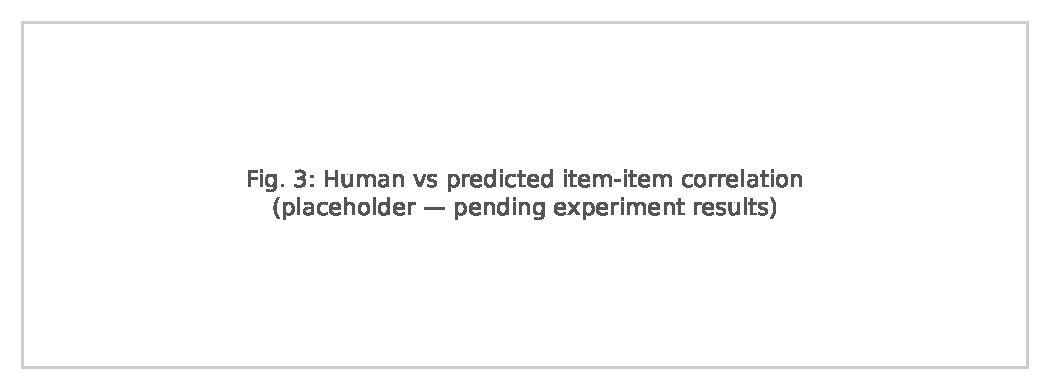
\includegraphics[width=0.98\columnwidth]{figures/fig3_correlation_heatmaps.pdf}
\caption{Human versus predicted (expected-score) item--item correlation
matrices at $K{=}5$ for Context QLoRA, P2P-Static, and RAP2P. \emph{Generated
by} \texttt{scripts/make\_figures.py}. Closer agreement with the leftmost
(human) panel indicates better joint-structure fidelity.}
\label{fig:heatmap}
\end{figure}

\subsection{Matched-Profile Heterogeneity (Table~\ref{tab:hetero})}
\label{sec:hetero}
This is the sharpest test of whether the model is more than a stereotype
machine. Pairs must satisfy both halves of the definition: (i) demographics
matched on age-bin/education/income-quintile/urbanicity (exact or at most one
mismatch), and (ii) known answers that \emph{actually diverge}---mean
normalized answer distance above a threshold over a canonical set of selection
items that are then \emph{excluded} from the target comparison, so the variable
used to select pairs never contaminates the outcome. We report the Spearman
correlation between predicted and true answer divergence, and a Divergence
Reproduction Ratio (DRR); DRR$\approx 0$ means the model collapses matched
pairs onto one answer, DRR$\approx 1$ means predicted divergence tracks true
divergence in magnitude.

\begin{table}[t]
\centering
\caption{Matched-Profile Heterogeneity at $K{=}5$ (ID test). \emph{Source:}
\texttt{artifacts/metrics/heterogeneity.csv} (columns \texttt{n\_pairs},
\texttt{spearman\_rho}, \texttt{drr}). Higher $\rho$ and DRR closer to $1$ are
better; the day-1 gate confirmed enough divergence-filtered pairs per domain.}
\label{tab:hetero}
\setlength{\tabcolsep}{5pt}
\begin{tabular}{lccc}
\toprule
Method & $n_{\mathrm{pairs}}$ & $\rho$ (pred vs.\ true)\,$\uparrow$ & DRR ($\to 1$) \\
\midrule
Context QLoRA  & [--] & [--] & [--] \\
P2P-Static     & [--] & [--] & [--] \\
\textbf{RAP2P} & [--] & [--] & [--] \\
\bottomrule
\end{tabular}
\end{table}

\subsection{Generalization and ablations (Table~\ref{tab:gen})}
\label{sec:ablations}
Table~\ref{tab:gen} reports accuracy at $K{=}5$ across the three
generalization axes, and the ablation ladder. Free ($\dagger$) ablations reuse
the primary RAP2P checkpoint with inference-time masking; retrained rows are
independently trained cross-checks.

\begin{table}[t]
\centering
\caption{Generalization (top) and ablations (bottom), accuracy at $K{=}5$
(macro domain). Generalization from \texttt{respondent\_macro\_seed\_mean.csv}
filtered to \texttt{split}$\in\{$\texttt{test}, \texttt{ood\_intersection}$\}$
and \texttt{item\_pool}$\in\{$\texttt{seen}, \texttt{unseen}$\}$. Ablation rows:
$\dagger$ = inference-time (free) mask on the primary RAP2P checkpoint; others
independently retrained. MIRT has no item parameters for unseen items (N/A).}
\label{tab:gen}
\setlength{\tabcolsep}{4pt}
\begin{tabular}{lccc}
\toprule
\multicolumn{4}{l}{\emph{Generalization (accuracy, $K{=}5$)}}\\
Method & ID Resp. & OOD Int. & OOD Item \\
\midrule
Demographic MIRT & [--] & [--] & N/A \\
Context QLoRA    & [--] & [--] & [--] \\
P2P-Static       & [--] & [--] & [--] \\
\textbf{RAP2P}   & [--] & [--] & [--] \\
\midrule
\multicolumn{4}{l}{\emph{Ablations (accuracy, $K{=}5$, ID test)}}\\
Variant & Acc & $\Delta$ vs.\ full & Removed \\
\midrule
RAP2P (full)             & [--] & ---  & --- \\
No demographics$^{\dagger}$ & [--] & [--] & prior \\
No history$^{\dagger}$      & [--] & [--] & anchoring \\
No history (retrained)   & [--] & [--] & cross-check \\
No corr.\ graph$^{\dagger}$ & [--] & [--] & $\gamma C_{jk}$ \\
noGraph (retrained)      & [--] & [--] & cross-check \\
Uniform gate$^{\dagger}$    & [--] & [--] & router \\
\bottomrule
\end{tabular}
\end{table}

\emph{[NOTE: consistency check---the ``$\dagger$ free'' and ``retrained'' rows
for no-history and no-corr-graph should be close. A large gap means the
modality-dropout scheme is not a faithful stand-in for a true retrain, in which
case report retrained numbers only.]}

\subsection{Option-order robustness (Table~\ref{tab:permutation})}
\begin{table}[t]
\centering
\caption{Permutation consistency at $K{=}5$ over five option-label
permutations (500-respondent subsample). \emph{Source:}
\texttt{artifacts/metrics/permutation\_consistency.csv}. Higher is more robust
to option-order framing effects.}
\label{tab:permutation}
\setlength{\tabcolsep}{5pt}
\begin{tabular}{lcc}
\toprule
Method & \# perm. & Consistency\,$\uparrow$ \\
\midrule
Local Sparse-ICL & 5 & [--] \\
Context QLoRA    & 5 & [--] \\
\textbf{RAP2P}   & 5 & [--] \\
\bottomrule
\end{tabular}
\end{table}

\section{Discussion}
\label{sec:discussion}

\paragraph{Claim-strength ladder.}
The strength of our claim is decided by the numbers, not chosen in advance. In
the \emph{strongest} outcome, RAP2P beats both Context QLoRA and P2P-Static on
accuracy, MAE, and NLL at $K\in\{3,5\}$ (Table~\ref{tab:main},
Table~\ref{tab:bootstrap}), \emph{and} on Group JS / CorrErr
(Table~\ref{tab:structure}), \emph{and} on Matched-Profile Heterogeneity
(Table~\ref{tab:hetero}); the full story is then that target-aware parameter
routing outperforms both in-context and static profile-to-parameter
personalization without sacrificing population structure. In an
\emph{acceptable} outcome, RAP2P ties Context QLoRA on raw accuracy but wins
clearly on OOD-intersection generalization and heterogeneity, supporting the
narrower claim that parameter-space personalization preserves within-group
heterogeneity more effectively than context-space personalization at lower
inference-time token cost and a fixed $64$-scalar per-user state. In the
\emph{unsupported} outcome, Context QLoRA matches or beats RAP2P on every axis,
which we would report plainly rather than re-running ablations until something
looks favorable.

\paragraph{What the classical baseline tells us.}
If Demographic MIRT is statistically indistinguishable from RAP2P at every $K$
(Table~\ref{tab:bootstrap}), the gain in this task comes from a classical
latent-trait prior--posterior update rather than from LLM item semantics or
target-aware routing---a legitimate, narrower finding that we would state
directly. The comparison is therefore not a strawman but a genuine test of
whether the LLM machinery earns its cost.

\section{Limitations}
\label{sec:limitations}
We state the scope cuts up front. First, there is \textbf{no cross-country
generalization axis}: SocioBench spans many countries, but we evaluate unseen
respondents, unseen demographic intersections, and unseen items, not unseen
countries. Second, we study \textbf{two domains, not ten}, chosen before
looking at any model result; the findings should not be extrapolated to all
SocioBench domains without further evidence. Third, the \textbf{income-quintile
binning assumes a specific ISSP scale direction}, which is load-bearing for the
OOD-intersection and heterogeneity axes and must be checked against each
domain's codebook. Fourth, \textbf{ordinal-item selection is an
English-keyword heuristic} whose false-negative rate we have not measured.
Fifth, \textbf{stratified splitting backs off to coarser strata for small
cells}, so the stated stratification is approximate for sparse combinations.
Sixth, the \textbf{MIRT baseline is a categorical simplification}, not a
graded-response model with ordered thresholds, so conclusions about
``classical IRT'' apply strictly to this variant. Seventh, \textbf{four of the
ablation rows come from one jointly trained checkpoint with inference-time
masking}; the two retrained cross-checks exist precisely to validate this
choice. Finally, this work produces probabilistic \emph{synthetic} survey
responses under explicit modeling assumptions---conditional answer
distributions, not digital twins of real people.

\section{Ethical Statement}
Synthetic survey respondents can lower the cost of pretesting instruments and
exploring counterfactual populations, but they also risk being mistaken for
real public opinion or used to manufacture the appearance of consensus. RAP2P
conditions on a small number of a real respondent's answers, which raises the
usual privacy considerations for panel data; all SocioBench data used here are
already de-identified and publicly released, and our item-holdout and
intersection-holdout guards prevent the model from memorizing held-out target
answers. We emphasize that the method estimates conditional answer
distributions under stated assumptions and is not a substitute for human
participants; results should not be reported as if collected from people.

% References
\bibliography{refs}

\end{document}
